\documentclass[tikz,border=8pt]{standalone}
\usepackage{amsmath}
\usetikzlibrary{arrows.meta,positioning}

\begin{document}
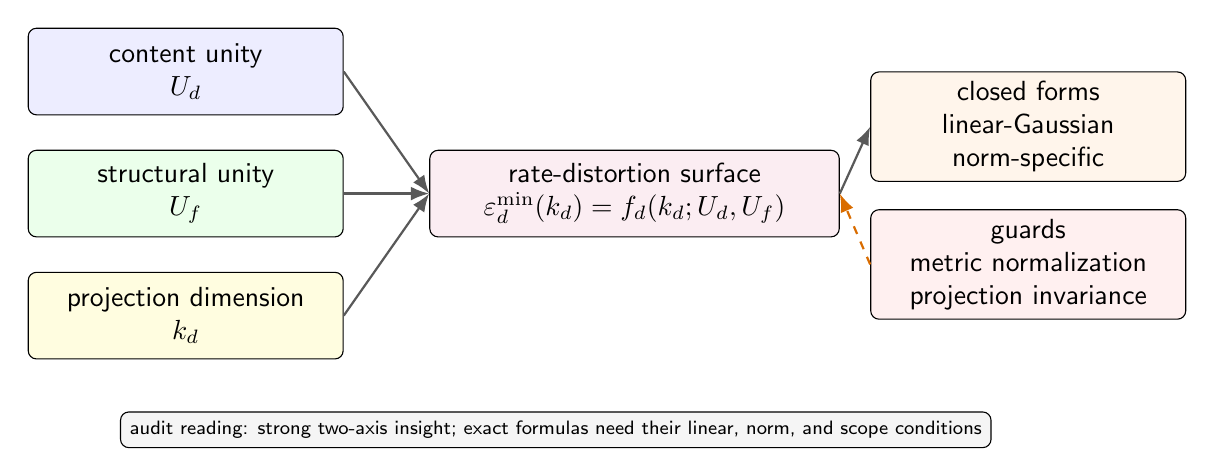
\begin{tikzpicture}[
  font=\sffamily,
  box/.style={draw, rounded corners=3pt, align=center, minimum width=40mm, minimum height=11mm, fill=white},
  note/.style={draw, rounded corners=3pt, align=center, font=\sffamily\scriptsize, fill=white},
  arrow/.style={-Latex, thick, draw=black!65},
  warn/.style={-Latex, thick, dashed, draw=orange!85!black}
]

\node[box, fill=blue!7] (content) at (-4.7,1.55)
  {content unity\\$U_d$};
\node[box, fill=green!8] (structure) at (-4.7,0)
  {structural unity\\$U_f$};
\node[box, fill=yellow!12] (dim) at (-4.7,-1.55)
  {projection dimension\\$k_d$};

\node[box, fill=purple!7, minimum width=52mm] (surface) at (1.0,0)
  {rate-distortion surface\\$\varepsilon_d^{\min}(k_d)=f_d(k_d;U_d,U_f)$};
\node[box, fill=orange!8] (closed) at (6.0,0.85)
  {closed forms\\linear-Gaussian\\norm-specific};
\node[box, fill=red!6] (guards) at (6.0,-0.9)
  {guards\\metric normalization\\projection invariance};

\draw[arrow] (content.east) -- (surface.west);
\draw[arrow] (structure.east) -- (surface.west);
\draw[arrow] (dim.east) -- (surface.west);
\draw[arrow] (surface.east) -- (closed.west);
\draw[warn] (guards.west) -- (surface.east);

\node[note, fill=gray!8, minimum width=78mm] at (0,-3.0)
  {audit reading: strong two-axis insight; exact formulas need their linear, norm, and scope conditions};

\end{tikzpicture}
\end{document}
